\chapter{Plotting}
\index{plotting}
\label{c:plotting}

\tao has a graphical display window within which such things as lattice functions, machine layout,
beam positions, etc., can be plotted. An example is shown in \fig{f:plot.typ} where there are plots
of the beta function and orbit along with a ``lattice layout which shows the longitudinal positions
of lattice elements. 

\tao uses a software toolkit called \vn{quick_plot} for plotting. Detailed information on this is in
section~\sref{s:quick.plot}.

\begin{figure}[b]
  \centering
  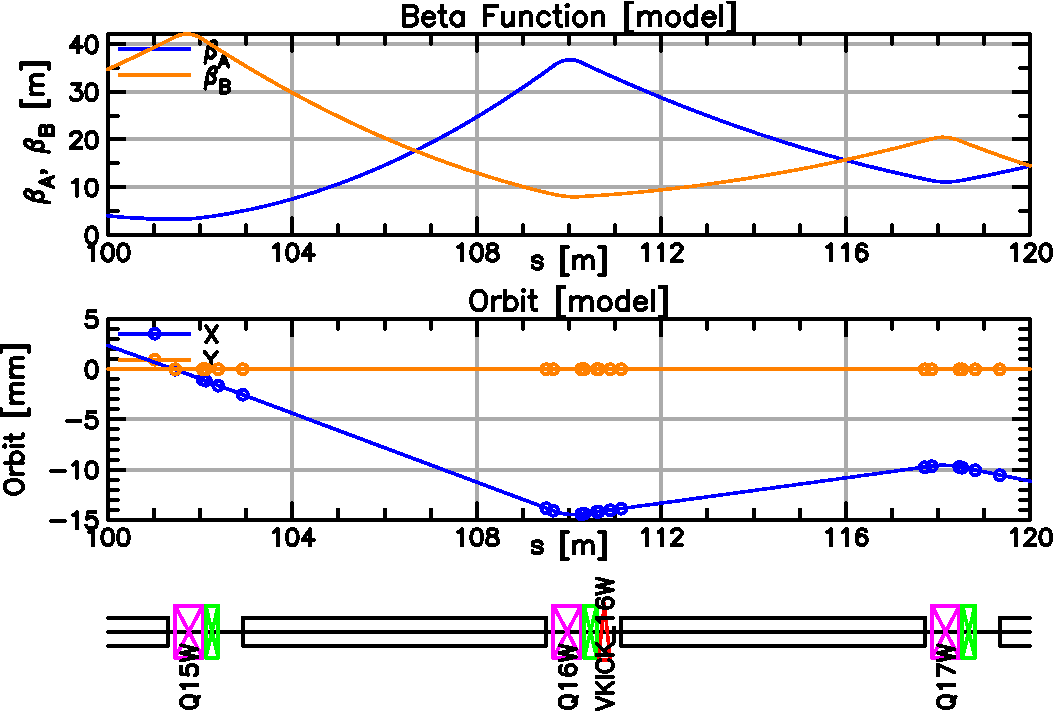
\includegraphics[width=5.0in]{plot-typical.pdf}
  \caption[An example of a plot display.]
{In this example there are three plot: A plot displaying the beta funciton, a plot displaying the
orbit, and a plot displaying the ``lattice layout'' which shows the longitudinal positions of
lattice elements.}
  \label{f:plot.typ}
\end{figure}

\begin{figure}[bt]
  \centering
  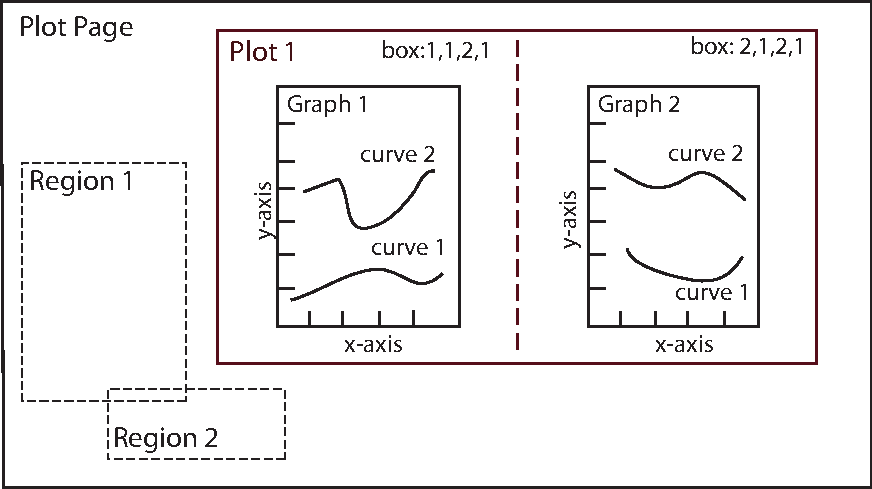
\includegraphics[width=5.0in]{plot.pdf}
  \caption[Plotting nomenclature.]
{The \vn{plot page}, which is the whole display window, has a number of rectangular \vn{regions} in
which a \vn{plot} can be placed. A plot has a collection of graphs and a graph has a collection of
curves. A plot template becomes visible when it is associated with some region on the page using the
\vn{place} command. Note that on the actual page the plot/region border is not visible.}
  \label{f:plot}
\end{figure}

%-----------------------------------------------------------------
\section{Plot Page}
\label{s:plot.page.def}

The \vn{plot page}, sometimes called the \vn{plot window}, refers to the window where graphics are
displayed or the corresponding printed graphics page. A \vn{plot page} is shown schematically in
\fig{f:plot}. Parameters associated with the \vn{plot page} are discussed in \sref{s:plot.page}.
These parameters may be set in an initialization file or may be set on the \tao command line using
the \vn{set plot_page} (\sref{s:set.plot.page}) command. Examples:
\begin{example}
  set plot_page text_height = 11  ! 11 point font size
  set plot_page border%x1 = 0.2   ! Set left page border to 20% of width.
\end{example}

The \vn{show plot -page} (\sref{s:show.plot}) command may be used to view the page paramteters.

%-----------------------------------------------------------------
\section{Region}
\label{s:region.def}

The \vn{plot page} is divided up into a number of rectangles called \vn{regions}. \vn{Regions}
define the locations where \vn{plots} may be placed. This is shown schematically in \fig{f:plot}
which shows two regions. Each region has a name and information on where the region is on the plot
page. Regions may be defined by the user. In addition, for convienience, \tao will define a number
of regions. With one exception, all of the \tao defined regions will begin with the letter
'r'. Regions may overlap. How to define regions is explained in \sref{s:plot.page}. The \vn{show
plot} command will show the region list. Example:
\begin{example}
  Tao> show plot

Plot Region         <-->  Plot                 x1    x2    y1    y2     Visible
-----------               -----------------------------------------------------
layout              <-->  lat_layout          0.00  1.00  0.00  0.15         T
r11                 <-->                      0.00  1.00  0.15  1.00
r12                 <-->                      0.00  1.00  0.58  1.00
r22                 <-->                      0.00  1.00  0.15  0.58
r13                 <-->  beta                0.00  1.00  0.72  1.00         T
r23                 <-->  dispersion          0.00  1.00  0.43  0.72         T
r33                 <-->  orbit               0.00  1.00  0.15  0.43         T
r14                 <-->                      0.00  1.00  0.79  1.00
\end{example}

The \vn{Plot} column shows what \vn{plot} (if any) is associated with the region (see below). The
next four columns define where the region rectagle is (\sref{s:plot.page}). Finally, the last column
shows if the \vn{plot} associated with the \vn{region} is visible. Normally everything is
visible. Invisibility is used in some special cases. For example, when using a Graphical User
Interface (GUI).

The \vn{set region} command can be used to set region parameters. Example:
\begin{example}
  set region r13 y1 = 0.8  ! Sets lower edge vertical position
\end{example}

%-----------------------------------------------------------------
\section{Plot}
\label{s:plot.def}

A \vn{plot} is essentially a collection of \vn{graphs}. This is shown schematically in \fig{f:plot}
which shows a plot with two graph and \fig{f:plot.typ} shows a plot page with three plots.

Plots are divided into two groups. A \vn{template} plot defines how a \vn{displayed} plot is to be
constructed. That is, a \vn{template} plot defines what the associated \vn{graphs} are, defines
graph placement, etc. When a \vn{template} plot is \vn{placed} in a \vn{region}, using the
\vn{place} command, the information of the \vn{template} is copied in order to construct a
\vn{displayed} plot. A given \vn{template} plot may be placed in multiple \vn{regions} to give
multiple \vn{displayed} plots and then, using \vn{set} commands, the data displayed in each of these
plots may be manipulated separately. For example, one displayed orbit plot could show the orbit of
the \vn{model} lattice while another orbit plot could show the orbit difference between the
\vn{model} and \vn{design} lattices. When a \vn{plot} is displayed in a given \vn{region},
everything drawn is scalled to the region size.

Use the \vn{show plot} to see what displayed plots are associated with what regions. Use the
\vn{show plot -templates} command to see a list of \vn{template} plots. \tao defines a number of
default \vn{template} plots. Section~\sref{s:templates} discussses how to define custom template
plots in an initialization file. Use the \vn{set plot} command to modify either \vn{template} or
\vn{displayed} plots.

All plots have a name. A \vn{displayed} plot will inherit the same name of the \vn{template} plot it
came from. If a given \vn{template} plot is used to create multiple \vn{displayed} plots. All of
these plots will have the same name. A \vn{displayed} plot can also be referred to by using the
associated \vn{region} name. This can be used to remove ambiguity if there are multiple \vn{displayed}
plots of the same name. Also a \vn{template} plot can unambiguously be referred to by adding the prefix
``\vn{T::}'' to the plot name. 

Some commands, for example, the \vn{scale} command by default will ignore \vn{template} plots unless
the plot name has the \vn{T::} prefix. Other commands, for example \vn{show plot} command, will
preferentially show displayed plot info but will show template plot info if there are not matching
displayed plots. Examples:
\begin{example}
  scale orbit -10 10    ! Scale all displayed orbit plots. Ignore template.
  scale r33 -10 10      ! Scale only plot in r33 region.
  scale T::orbit -10 10 ! Scale template orbit plot.
  show plot e_field     ! Will show displayed e_field plot info. If no
                        ! displayed plot exists, will show template info.
\end{example}


%-----------------------------------------------------------------
\section{Box}
\label{s:box.def}

To determine where a \vn{graph} is drawn with respect to the boundaries of its associated \vn{plot},
each \vn{graph} is associated with a given \vn{box}. A \vn{box} is a rectangular sub-region of the
\vn{plot}. Boxes are defined by dividing the \vn{plot} into a rectangular grid and then choosing one
of the grid rectagles to be the \vn{box} associated with the \vn{graph}. The is illustrated in
\fig{f:plot} where \vn{Graph 1} of \vn{Plot 1} is associated with the box with label
``\vn{1,1,2,1}''.  The last two digits of a \vn{box} label (\vn{2,1} here) specify the number of
rectangles grid has horizontally and vertically (2 horizontally, 1 vertically here). The first two
digits (\vn{1,1} here) specify the particular rectangle associated with the \vn{box} with \vn{1,1}
designating the lower left rectangle. Different \vn{graphs} do not have to use the same grid to
select a box from.

Setting the \vn{box} for a given \vn{graph} in a \tao initalization file is covered in \sref{s:template}.
The \vn{set graph} and \vn{show graph} commands can be used to set and show the box parameters. 
Examples:
\begin{example}
  set graph myplot.g1 box = 2 1 2 2  ! Set box of graph myplot.g1
  set graph myplot.g2 box = 1 1 1 2  ! Different graphs can use differnet grids
                                     !  for box selection
  set graph orbit.g curve_legend_origin = 0.1 -0.2 "%BOX/LT"  ! Set curve legend origin
\end{example}
The last example sets the \vn{curve legend} (\sref{s:template}) of the graph so that the curve
legend of the graph is drawn with respect to the left top corner of the box.

%-----------------------------------------------------------------
\section{Graph}
\label{s:graph.def}

A \vn{graph} is a diagram of some sort.  Most \vn{graph}s consists of horizontal and vertical axes
along with one or more \vn{curve}s. \vn{Floor_plan} (\sref{s:floor.plan}) and \vn{lat_layout}
\vn{graphs}, on the other hand, shows the placement in space of the lattice elements and do not have
any associated \vn{curves}. A given \vn{plot} will contain a number of \vn{graphs}. For example, in
\fig{s:plot} the plot labeled \vn{plot 1} is shown to have two graphs.

How many \vn{graphs} is assocaited with a \vn{plot} is a matter of convienience and different
\vn{graphs} of a \vn{plot} may display different types of information. For example, it would be
possible to have a single \vn{plot} contain three \vn{graphs} and look like what is shown in
\fig{f:plot.typ}. In actuality, the figure was constructed using three \vn{plots} each one containing
one \vn{graph}.

All graphs have a name. For example, the graph of the standard \vn{orbit} plot is simply ``\vn{g}''.
\vn{Graphs} may be referred to using the syntax:
\begin{example}
  <plot>.<graph>
\end{example}
where \vn{<plot>} is the plot name and \vn{<graph>} is the graph name. If the \vn{.<graph>} ending
is omitted, all graphs of the named \vn{plot}(s) are selected. Examples:
\begin{example}
  show graph beta   ! Show info of all graphs in all the displayed beta plots.
  show graph r13.g1 ! Show info on ``g1'' graph of region r13.
\end{example}

How to define \vn{graphs} when defining \vn{template} plots is given in \sref{s:template}. The
\vn{show graph} command can be used to show graph parameters. The \vn{set graph} command can
be used to modify \vn{graph} parameters.

%-----------------------------------------------------------------
\section{Curve}
\label{s:curve.def}

A \vn{curve} is a data set to be displayed within a \vn{graph}. For example, a \vn{curve} may be the
beta function of the \vn{model} lattice. \vn{Curves} have an associated set of points at which a
symbol can be drawn and/or a curved line that can be drawn. For example, in \fig{f:plot.typ} only
the line is drawn with the two curves of the beta plot while both symbols and line are drawn for the
two curves of the orbit plot (here the data points are the orbit at the edges of the lattice elements).

All curves have a name. \vn{Curves} may be referred to using the syntax:
\begin{example}
  <plot>.<graph>.<curve>
\end{example}
where \vn{<plot>} is the plot name, \vn{<graph>} is the graph name and \vn{<curve>} is the curve
name. If the \vn{.<curve>} ending is omitted, all curves of the named \vn{graph}(s) are
selected. If the \vn{.<graph>.<curve>} ending is omitted, all curves of the named \vn{plot}(s) are
selected. Examples:
\begin{example}
  show curve beta   ! Show info of all curves in all the displayed beta plots.
  show curve r13.g1 ! Show info on curves in ``g1'' graph of region r13.
\end{example}

How to define \vn{curves} when defining \vn{template} plots is given in \sref{s:template}. The
\vn{show curve} command can be used to show curve parameters. The \vn{set curve} command can
be used to modify \vn{curve} parameters.


* component

* symbols and lines

* which data is displayed: graph%draw_only_good_user_data_or_vars 

* smooth line calc.

* Clipping.

%-----------------------------------------------------------------
\section{Graph Types}
\label{s:graph.types}

\tao defines several kinds of graphs
\begin{description}
%
\item[\vn{Data Graph}] \Newline
``Data'' plotting here has a specific meaning. That is, the plotting of a dependent variable on the
$y$-axis vs an independent variable on the $x$-axis. Typically the independent variable
will be the longitudinal position $s$-position as in the upper two graphs in \fig{s:plot.typ}. Also
see \Sref{s:draw.ap} for an example where beam apertures are added to the graph.

%
\item[\vn{Data Slice Graph}] \Newline
A ``\vn{data slice}'' graph is plotting one data array on the $y$-axis versus another data array on
the $x$-axis.

%
\item[\vn{}] \Newline

%
\item[\vn{}] \Newline

%
\item[\vn{}] \Newline

%
\item[\vn{}] \Newline

%
\item[\vn{}] \Newline


\end{description}

data plot with apertures
Dynamic apertures
floor_plan
histograph
key table, 
lat_layout
phase space

%-----------------------------------------------------------------
\section{Graph Axes}
\label{s:axes}

* x2 and y2

* x-axis types



%-----------------------------------------------------------------
\section{Quick_Plot Plotting}
\label{s:quick.plot}

\vn{Quick_plot} is an interface library developed for \bmad for graphics plotting. 

QuickPlot uses
the following concepts:
\begin{example}
  PAGE  -- The entire drawing surface.
  PLOT  -- A rectangle defined with respect to the PAGE within which graphs are placed.
  BOX   -- For each GRAPH associated with a given PLOT, the GRAPH defines a two-dimensional array of BOXes that
            partition the PLOT. The GRAPH is positioned with respect to a given BOX in this array. 
            Each GRAPH can define a different two-dimensional array of B0Xes.
  GRAPH -- The actual plotting rectangle where curves are drawn within the bounds of the axes.
\end{example}

%-----------------------------------------------------------------
\subsection{Length and Position Units}
\label{s:qp.units}

Positions and lengths with \vn{quick_plot} generall have an associated ``\vn{units}'' string which determines how
$(x, y)$ positions or $(dx, dy)$ lengths are to be interpreted. 
The syntax of the \vn{units} parameter is:
\begin{example}
   "unit_type/ref_object/corner"
\end{example}
A \vn{units} string has a \vn{unit_type}, \vn{ref_object} and \vn{corner} components separated by slashes ``/''.

The \vn{unit_type} component is the type of units which can be one of:
\begin{example}
   "%"       - Percent.
   "DATA"    - Data units associated with a graph.
   "MM"      - millimeters.
   "INCH"    - Inches.
   "POINTS"  - Printers points (72 points = 1 inch, 1 pt ~ 1 pixel).
\end{example}
Note: If \vn{unit_type} is set to \vn{"DATA"}, \vn{ref_object}, if present, must be \vn{"GRAPH"} and
\vn{corner}, if present, must be \vn{"LB"}.

The \vn{ref_object} component is a reference object which can be one of:
\begin{example}
   "PAGE"  -- Relative to the plot display window.
   "BOX"   -- Relative to the box the graph is associated with.
   "GRAPH" -- Relative to the graph rectangle.
\end{example}
The \vn{ref_object} component is optional if a relative length is being specified and the
\vn{unit_type} is anything other than \vn, the slash between
the \vn{unit_type} and the \vn{ref_object} may be omitted.

And the \vn{corner} component is the origin location of the reference object.
\vn{corner} can be one of:
\begin{example}
   "LB" -- Left Bottom of reference object. Default.
   "LT" -- Left Top.
   "RB" -- Right Bottom.
   "RT" -- Right Top.
\end{example}
The \vn{ref_object} component is optional if a relative length is being specified.

Examples:
\begin{example}
  "DATA"          -- Equivalent to "DATA/GRAPH/LB"
  "DATA/GRAPH/LB" -- Same as above.
  "DATA/BOX/RT"   -- ILLEGAL: DATA must always go with GRAPH/LB.
  "%/PAGE/LT"     -- Equivalent to "%PAGE/LT"
  "%PAGE/LT"      -- Percentage of page so (0.0, 1.0) = RT of page.
  "%BOX"          -- Percentage of box so (1.0, 1.0) = RT of box.
  "INCH/PAGE"     -- Inches from LB of page. Equivalent to "INCH/PAGE/LB"
\end{example}

Units can be set in an initialization file or with the \vn{set} command. Example:
\begin{example}
  set plot_page title%units = '%PAGE'
\end{example}

%-----------------------------------------------------------------
\subsection{Text Justification Units}
\label{s:qp.str.just}

Text justification units is a two character string that sets where a line of text is to be printed
with respect to the text $(x, y)$ position.
The first character of the justification string gives the horizontal alignment:
\begin{example}
   "L" -- Left justify
   "C" -- Center justify
   "R" -- Right justify
\end{example}
The second character of the justification string gives the vertical alignment:
\begin{example}
   "B" -- Bottom justify
   "C" -- Center justify
   "T" -- Top justify
\end{example}

Example:
\begin{example}
  plot_page%title%justify = 'CC'
\end{example}

%-----------------------------------------------------------------
\subsection{qp\_point\_struct}
\label{s:qp.point}

\vn{QuickPlot} defines a number of structures to parameterize such things like line and symbol
properties.

The \vn{qp_point_struct} defines where a point is:
\begin{example}
  type qp_point_struct:
    x     = <real>     ! Horzontal offset of point from fiducial point
    y     = <real>     ! Vertical offset of point from fiducial point
    units = "<units>"  ! Units of x \& y (\sref{s:qp.units}).
\end{example}
Example:
\begin{example}
  graph%curve_legend_origin = 5.0, -2.0, "POINTS/GRAPH/LT"
\end{example}
In this example the fiducial point the left-top point on the graph rectangle. The
\vn{curve_legend_origin} is positioned 5.0 points horizontally to the left and 2.0 points vertically
downward from this fiducial point.

%-----------------------------------------------------------------
\subsection{qp\_line\_struct}
\label{s:qp.line}

The parameters associated with data lines drawn in a graph are contained in the \vn{qp_line_struct}:
\begin{example}
  type qp_line_struct:
    width    = <integer>  ! Default = 1
    color    = <string>   ! Default = "black" (\sref{s:qp.color}).
    pattern  = <string>   ! Default = "solid" (\sref{s:qp.pattern}).
\end{example}

%-----------------------------------------------------------------
\subsection{qp\_symbol\_struct}
\label{s:qp.sym}

The parameters associated with symbols that are drawn are contained in the \vn{qp_symbol_struct}:
\begin{example}
  type qp_symbol_struct:
    type          = <string>  ! Default = "dot"
    height        = <real>    ! Size in points. Default = 10
    color         = <string>  ! Default = "black" (\sref{s:qp.color})
    fill_pattern  = <string>  ! Default = "solid_fill"
    line_width    = <integer> ! Default = 1.
\end{example}

%-----------------------------------------------------------------
\subsection{qp\_axis\_struct}
\label{s:qp.axis}

The \vn{qp_axis_struct} structure defines the properties of a graph axis
\begin{example}
  type qp_axis_struct::
    label             = "<string>" ! Axis label string.
    min               = <real>     ! Min is the left or bottom axis number.
    max               = <real>     ! Max is the right or top axis number.
    number_offset     = <real>     ! Offset from axis line in inches.
    label_offset      = <real>     ! Offset from numbers in inches.
    major_tick_len    = <real>     ! Major tick length in inches.
    minor_tick_len    = <real>     ! Minor tick length in inches.
    label_color       = <string>   ! Color of the label string (\sref{s:qp.color})
    major_div         = <integer>  ! Number of major divisions
    major_div_nominal = <integer>  ! Major divisions nominal value.
    minor_div         = <integer>  ! Minor divisions. 0 = Tao will choose.
    minor_div_max     = <integer>  ! Max minor div number if Tao chooses.
    places            = <integer>  ! Number of digits to print
    type              = <string>   ! Axis type: "LINEAR" or "LOG".
    bounds            = <string>   ! Axis bounds: "GENERAL", "ZERO_AT_END", etc.
    tick_side         = <integer>  ! 1 = draw to the inside, 0 = both, -1 = outside.
    number_side       = <integer>  ! 1 = draw to the inside, -1 = outside.
    draw_label        = <logical>  ! Draw the label string
    draw_numbers      = <logical>  ! Draw the numbers.
\end{example}

The \vn{%bounds} parameter sets how the axes min and max values are calculated when plots are initially
instantiated and when \vn{scale}, \vn{x_scale}, and \vn{xy_scale} commands are used. Possible settings
are:
\begin{example}
  "ZERO_AT_END"      ! Min or max value is set to zero.
  "ZERO_SYMMETRIC"   ! Min and max chosen so that max = -min.
  "GENERAL"          ! No restrictions (default).
  "EXACT"            ! The User min/max is used.
\end{example}
If input min and max values are specified by the User, \tao will take the specified values as the starting
point to find ``nice'' min and max values to use. For example, with the command
\begin{example}
  scale all 0 19
\end{example}
and with \vn{bounds} set to \vn{"GENERAL"}, the min and max values will be set to 0 and 20. The exception is when
\vn{bounds} is set to \vn{"EXACT"}. In this case the User supplied min and max values will be used as is.

Examples:
\begin{example}
Tao> set graph r13 y%bounds = "zero_at_end"
Tao> scale r13 200 280   ! Graph bounds set to [0, 300]

Tao> set graph r13 y%bounds = "zero_symmetric"
Tao> scale r13 200 280   ! Graph bounds set to [-300, 300]

Tao> set graph r13 y%bounds = "general"
Tao> scale r13 20 190    ! Graph bounds set to [0, 200]

Tao> set graph r13 y2%bounds = "exact"
Tao> scale r13 -y2 20 190    ! Y2 graph bounds set to [20, 190]
\end{example}

The \vn{major_div} parameter is not settable directly. Rather, \vn{major_div_nominal} may be set by
the user and then \tao will calculate the value of \vn{major_div} such that the value of
\vn{major_div} is ``close'' to the value of \vn{major_div_nominal} with the constraint that the value
of \vn{major_div} ``nicely'' divides the range from given by the values for \vn{min} and \vn{max}.

The \vn{places} parameter set the number of places to display a number. \tao will automatically
calculate this number and it is not user settable.

The \vn{label} parameter may include Greek letters, subscripts, superscripts, and special characters.
Encoding for these are given in Table~\ref{t:plot.escape}. 

%-----------------------------------------------------------------
\subsection{String Escape Sequencies}
\label{s:qp.point}

\begin{table}[tb]
\begin{tabular}{ll} \toprule
{\B}u       & Start a superscript or end a subscript \\[0.3ex]
{\B}d       & Start a subscript or end a superscript.
              {\B}u and {\B}d must always be used in pairs \\[0.3ex]
{\B}b       & Backspace (i.e., do not advance text pointer  
               after plotting the previous character) \\[0.3ex]
{\B}fn      & Switch to Normal font (1)       \\[0.3ex]
{\B}fr      & Switch to Roman font (2)        \\[0.3ex]
{\B}fi      & Switch to Italic font (3)       \\[0.3ex]
{\B}fs      & Switch to Script font (4)       \\[0.3ex]
{\B}{\B}    & Backslash character (\B)        \\[0.3ex]
{\B}x       & Multiplication sign ($\times$)  \\[0.3ex]
{\B}.       & Centered dot ($\cdot$)          \\[0.3ex]
{\B}A       & Angstrom symbol (\AA)         \\[0.3ex]
{\B}gx      & Greek letter corresponding to roman letter x. See Table~\ref{t:greek}. \\[0.3ex]
{\B}mN {\B}mNN & Graph marker number \vn{N} or \vn{NN} (1-31) \\[1ex]
{\B}(NNNN)  & 
\parbox{5.2in} {Character number NNNN (1 to 4 decimal digits) from the Hershey character set which
includes a number of special characters including mathematical, musical, astronomical, and
cartographical symbols.} \\ \bottomrule
\end{tabular}
\caption{Escape Sequences for Labels.}
\label{t:plot.escape}
\end{table}

Table~\ref{t:greek} shows how the character string \vn{"{\B}g<r>"}, where \vn{"<r>"} 
is a Roman letter, map onto the Greek character set.
\begin{table}[tb]
  \centering
  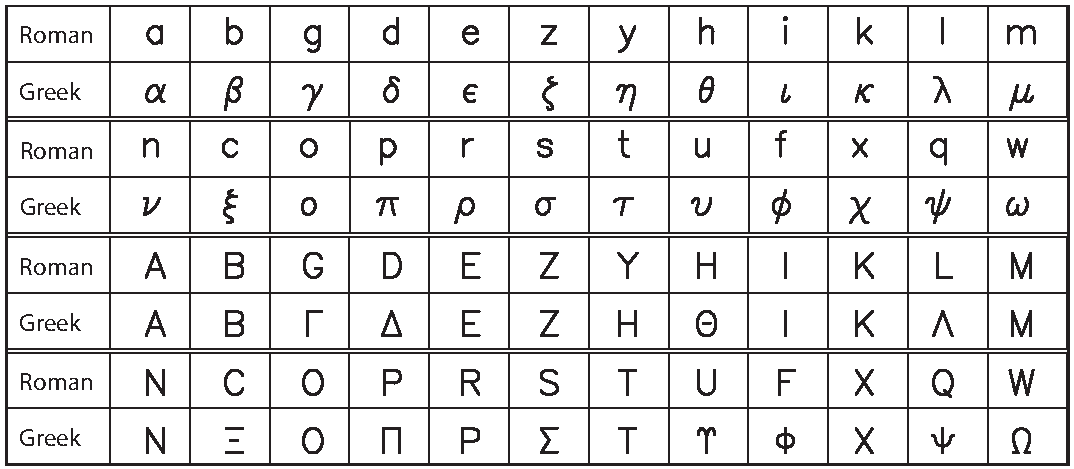
\includegraphics[width=5.0in]{greek.pdf}
  \caption[Roman to Greek Character Conversion]{Conversion for the string 
\vn{"{\B}g<r>"} where \vn{"<r>"} is a Roman character to the corresponding 
Greek character.}
\label{t:greek}
\end{table}

%-----------------------------------------------------------------
\subsection{Color Names}
\label{s:qp.color}

Possible settings for color parameters are:
\begin{example}
  White   (actually the background color)       Orange          
  Black   (actually the foreground color)       Yellow_Green    
  Red                                           Light_Green         
  Green                                         Navy_Blue       
  Blue                                          Purple          
  Cyan                                          Reddish_Purple  
  Magenta                                       Dark_Grey        
  Yellow                                        Light_Grey       
\end{example}
Color names are case insensitive.

%-----------------------------------------------------------------
\subsection{Line Pattern Names}
\label{s:qp.line.pat}

Possible settings for line patterns are:
\begin{example}
  solid      ! Solid line                 dotted     ! Dotted line             
  dashed     ! Dashed line                dash_dot3  ! Dash--dot--dot--dot line
  dash_dot   ! Dash--dot line
\end{example}
Pattern names are case insensitive.

%-----------------------------------------------------------------
\subsection{Fill Pattern Names}
\label{s:qp.fill.pat}

Possible fill pattern settings for symbols are:
\begin{example}
  solid_fill                    hatched           
  no_fill                       cross_hatched     
\end{example}
Fill pattern names are case insensitive.

%-----------------------------------------------------------------
\subsection{Symbol Names}
\label{s:qp.sym}

\begin{table}
  \centering
  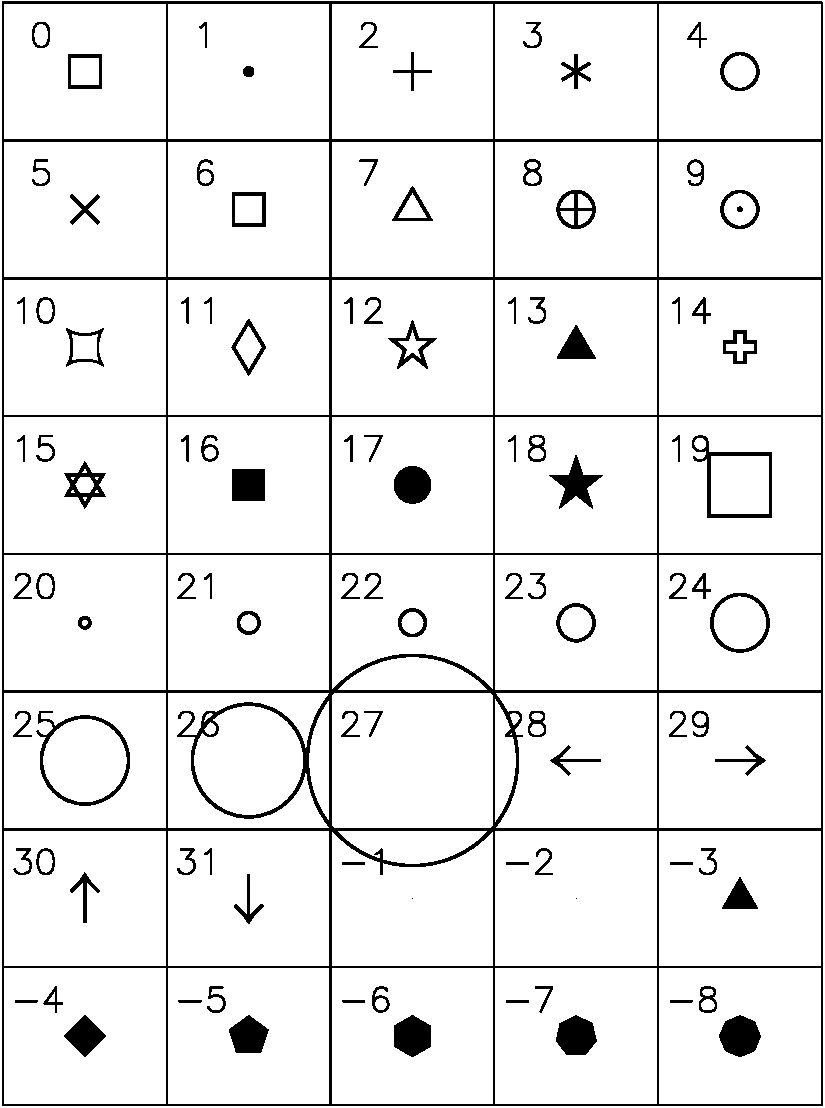
\includegraphics[width=5in]{plot-syms.pdf}
  \caption{Plotting Symbols.}
  \label{t:plot.syms}
\end{table}

The symbol types are:
\begin{example}
  square                 triangle                    square_concave              
  dot                    circle_plus                 diamond                     
  plus                   circle_dot                  star5                       
  times                  square_filled               triangle_filled           
  circle                 circle_filled               red_cross                 
  x                      star5_filled                star_of_david             
\end{example}
These symbols are illustrated in Table~\ref{t:plot.syms}. Symbol type names are case insensitive.

